%
% main.tex - a typical phil presentation
%
% Copyright (c) 2015, Phil Maker
% GPLv2 
% 
%    

\documentclass{beamer}
%\documentclass[a4paper,handout]{beamer}
%\usepackage{pgfpages}
%\pgfpagesuselayout{6 on 1}[a4paper,border shrink=5mm]

\mode<presentation>{\usetheme{Pjm}}
\usepackage{graphics}
\usepackage{fancyvrb}
\newenvironment{code}
{\Verbatim[fontfamily=courier,%
numbers=right,stepnumber=5,%
firstnumber=\the\inputlineno]}%
{\endVerbatim}
\usepackage[english]{babel}
%\usepackage[latin1]{inputenc}
\usepackage{hyperref}
\definecolor{links}{HTML}{2A1B81}
\hypersetup{
  pdftitle = {PV Diesel 101},
  pdfsubject = {PV Diesel}
  pdfkeywords = {Energy, Renewables, Powerwater, Phil Maker},
  pdfauthor = {\textcopyright\ Phil Maker, ...},
  pdfcreator = {\LaTeX\ with package \flqq hyperref \frqq},
  colorlinks,linkcolor=,urlcolor=links
}
\usepackage{xcolor}
\definecolor{JungleGreen}{cmyk}{0.99,0,0.52,0}
\definecolor{BlueGreen}{cmyk}{0.85,0,0.33,0}
\definecolor{RawSienna}{cmyk}{0,0.72,1,0.45}
\def\dill#1{\textcolor{RawSienna}{\textbf{Dill Alert: #1}}}

% select various versions
\usepackage{comment}
\excludecomment{nt-solar-concentrators}
\includecomment{nt-tkln}

\title{PV Diesel 101}
\author{Phil Maker
  \href{mailto:philip.maker@gmail.com}{\texttt{<philip.maker@gmail.com>}}
}
\institute{Powerwater Remote Operations/ACEP}
\date{March 2014}
\logo{
\includegraphics[height=0.7cm]{logo.jpg}}
\begin{document}

\begin{frame}
  \maketitle
  \vspace{-1.2cm}
  \begin{abstract}
    \small An introduction to PV Diesel Systems including principles
    of operation for medium and high penetration systems.
  \end{abstract}
\end{frame}

\section{Overview}
\begin{frame}\frametitle{Overview}
  This talk covers:
  \begin{itemize}
  \item Electricity, PV, Diesel, Control.
  \item How PV/Diesel Systems can be applied in isolated grids.
  \end{itemize}
  \pause
  It is \emph{not} about::

  \begin{itemize}
  \item Procurement, Kit, ....
  \item Operations,...
  \end{itemize}

  \pause
  There will be another chat about that, this is why and how not what..
  \vfill
  \begin{quote}
    ``There had been certain difficulties during
    the expedition and afterwards, There was
    no use denying it, I had simply told the
    story from my own point of view, as
    honestly as I could'' -– Tenzing Norgay.     
  \end{quote}
\end{frame}

\begin{frame}\frametitle{Conventions and References}
  \begin{itemize}
  \item \href{http://www.powerwater.com.au/solardiesel}{Solar
      Diesel Handbook} - a handbook about this topic.
    \pause
  \item \href{http://www.powerwater.com.au/solardiesel}{ASIM} - a
    simulator for PV Hybrid Systems (also see HOMER).
    \pause
  \item Naming conventions are as for ASIM: 
    \begin{itemize}
    \item Pv = Photo Voltaic, Gen = Generator, Load = Load, ...
    \item P = power, Q = reactive power, I = current
    \end{itemize}
    So what is:
    \begin{itemize}
    \item \texttt{Gen3P}, \texttt{GenP}, ...
    \item \texttt{PvSetP}, \texttt{Gen2I3}
    \end{itemize}
    \pause 
  \item See also Ackermann for Wind Diesel Hybrid Systems.
  \end{itemize}
\end{frame}

\begin{frame}\frametitle{Penetration and Contribution}
  \begin{itemize}
  \item \textbf{Power (kW)}, i.e. what is being used/generated now.
    \pause
    \begin{enumerate}
    \item Generation and Loads must balance: \texttt{GenP + PvP = LoadP}
    \item \textbf{Instantaneous Penetration} is the 
      \% of renewable power (kW) at this time: \texttt{100 * PvP/LoadP}
    \end{enumerate}
    \pause
  \item \textbf{Energy (kWh)}, i.e. what power has been used over a
    period.
    \pause
    \begin{enumerate}
    \item Over any period kWh must balance.
    \item \textbf{Average Penetration} is the \% of renewable energy
      (kWh) over a period (typically year): \texttt{100 * PvE/LoadE}
    \end{enumerate}
    \pause
  \item So a system with a \textbf{Peak Instantaneous Penetration} of
    60\% might result in an \textbf{Average Penetration} of 15\%.
  \item \textbf{Penetration} is also known as \textbf{Contribution}
    \pause
  \end{itemize}
  \dill{never confuse peak with average or kW and kWh!}

\end{frame}

\begin{frame}\frametitle{It is not all just about kW}
  \begin{itemize}
  \item \textbf{Frequency (Hz)}, typically ranging from 49 to 51Hz.
    (cycles per second for the boffins).
  \item \textbf{Voltage (V)}, typically 430V, for the hydro analogy
    this is height.
  \item \textbf{Current (I)}, for the hydro analogy this is flow rate.
    \pause
  \item \textbf{Reactive Power (vars)}, regulates the voltage, similar
    to kW it must balance:
    
    \texttt{GenQ = LoadQ}
  \end{itemize}
  Note that:
  \begin{itemize}
  \item If \texttt{(GenP or PvP > LoadP} then \texttt{F} increases.
  \item And vice versa
  \item Similarly for \texttt{Q} and \texttt{V}.
  \end{itemize}
\end{frame}

\begin{frame}\frametitle{PV good days and bad days}
  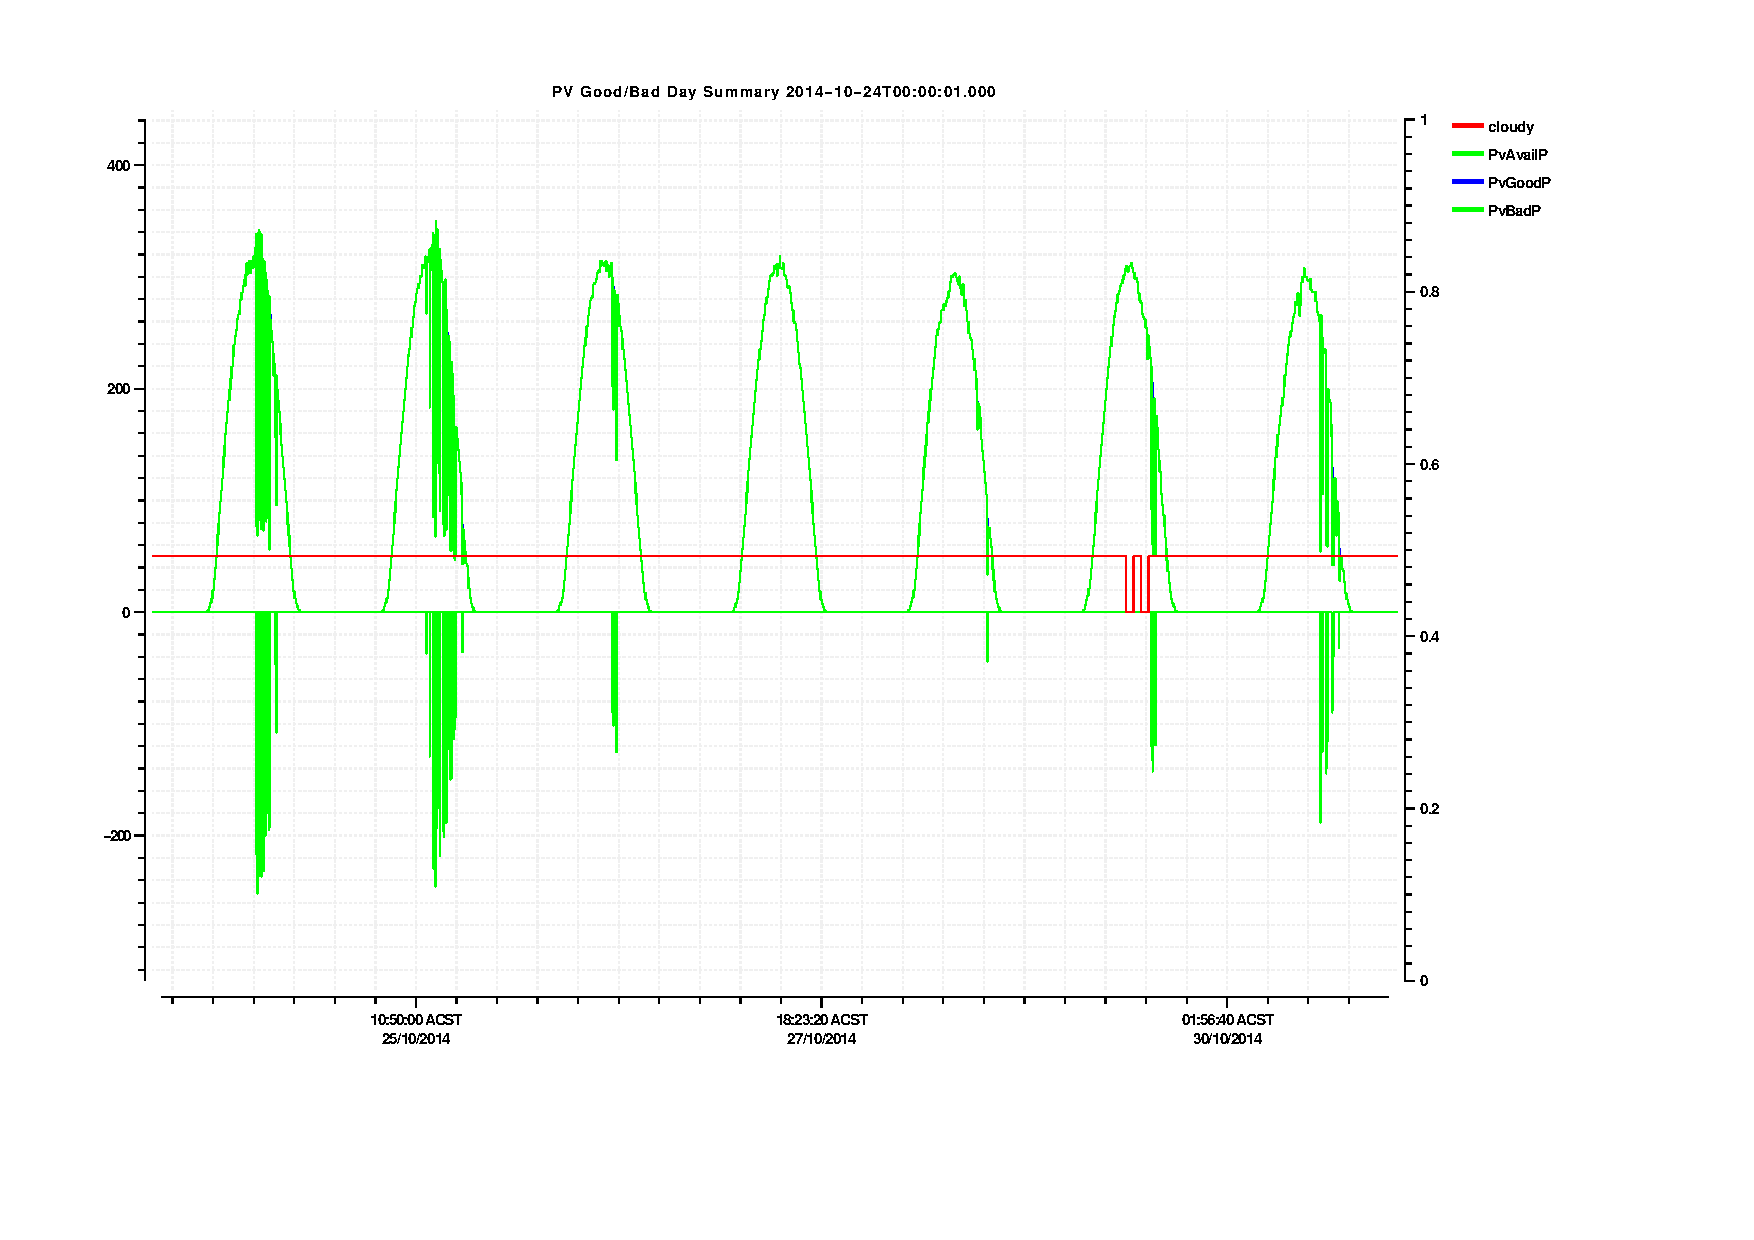
\includegraphics[width=12cm]{stuff/gday.pdf}
\end{frame}

\begin{frame}\frametitle{Capacity factor, Spinning Reserve, Step Load}
  \begin{itemize}
  \item \textbf{Capacity Factor}: is the energy generated divided by the
    energy it would have generated at full power over a period.
    \pause
    \begin{enumerate}
    \item PV: 20\% since the sun doesn't shine all the time.
    \item Wind: typically 25\% up to 57\% 
    \item US Coal is 63\%, U.S. Nuclear is 93\%.
    \item Three Gorges dam is around 50\%.
    \end{enumerate}
    \pause
  \item \textbf{Spinning Reserve}: the available spare power
    in the system: 
    \texttt{SpinP = GenMaxP - GenP}
    \pause
  \item \textbf{Step Load}: the capability to take a single
    immediate increase in load. Typically: 

    \texttt{StepP $<$ SpinP}
  \end{itemize}
\end{frame}

\begin{frame}\frametitle{Sharing: Droop, Isochronous and Setpoints}
Consider a two generator example:\pause
  \begin{itemize}
  \item Everything has to balance: \texttt{Gen1P + Gen2P = LoadP}\pause
  \item Load must be shared between generators: 
    \texttt{Gen1P/Gen1MaxP near Gen2P/Gen2MaxP}
  \end{itemize}
  This can be achieved by:
  \begin{itemize}
  \item \textbf{Droop:} uses frequency to communicate load, e.g.
    49.5Hz generator runs at 100\% capacity, at 50.5Hz it runs at 0\%.
    \pause
  \item \textbf{Isochronous}: uses a separate load sharing line 
    so that each generator can share whilst keeping frequency around
    50Hz.\pause
  \item \textbf{Setpoint control}: can be used to control output of
    devices but we need a mixture of Droop and Isochronous in order to
    balance the system.
  \end{itemize}
\end{frame}

\section{No Penetration}
\begin{frame}\frametitle{No Penetration PV}
  \begin{itemize}
  \item Start and stop diesel in order to keep:
    
    \texttt{SpinP > SpinMinPPa}
  \item For a 500kW system \texttt{SpinMinPPa} might
    be 30kW. It is typically the largest load in town.  \pause
  \item Always try to run the smallest set possible but:
    \begin{itemize}
    \item Always run a set for perhaps 30 minutes after starting it.
    \item Switch down only after the load has gone down a bit further
      (\texttt hysterisis).
    \item Many other things...
    \end{itemize}
    \pause
  \item Generator sizes need to selected based on load.
    \begin{itemize}
    \item Either all the same and run them together.
    \item All different, e.g. small, medium and large.
    \end{itemize}
    \pause
  \item Generators have to be loaded properly (both low and high).
  \end{itemize}
  \pause
  \dill{Lets replace Station X with 2 x 1MW containerised sets where 
  load varies from 500..1400 kW}
\end{frame}

\section{Low Penetration}
\begin{frame}\frametitle{Low Penetration PV}
  \begin{itemize}
  \item No control of PV, just let it run at full power all the time.
    \pause
  \item Depend on the normal spinning reserve to handle
    cloud events. Typical generator start times are around 1 minute.
    \pause
    \dill{PV varies once every minute for data sampled once 
      every minute}
    \pause
  \item A bad cloud event typically takes 10s, e.g.
    \begin{enumerate}
    \item Wind speed at 1000m = 5m/s
    \item Field is 50m across.
    \item Result is obvious, i.e. PV variability depends on wind speed.
    \end{enumerate}
  \item Low Penetration is limited to 10..20\% (spinning reserve).
  \end{itemize}
  \dill{Design a power system where we keep 30kW of
    Spinning Reserve and try to install 60kW of PV.}
\end{frame}

\section{Medium Penetration}
\begin{frame}\frametitle{Medium Penetration PV}
Medium penetration systems typically do not use storage and
reach a peak penetration of perhaps 60\% for a 40\% minimum generator
loading.
\pause
  \begin{enumerate}
  \item Active control of generation and PV in order to maintain:
    
    \texttt{PvP <= SpinP}

    So if all the PV disappears before we can start a diesel we will
    be alright.
    \pause
  \item We also need to maintain diesel loading above a threshold:
    
    \texttt{GenP >= GenMinP}

    In order to avoid damage to diesel generation.
    \pause
  \item So control:\texttt{GenMaxP} and \texttt{PvSetP} in order to
    meet 1 and 2.
  \end{enumerate}
\end{frame}

\begin{frame}\frametitle{Medium Penetration Example}
  \begin{itemize}
  \item Keep enough spinning reserve online: 

    \texttt{GenMaxP >= GenP + max(PvP,GenSpinPPa)}
   \pause
  \item So loss of 100\% of the Pv over 10s will be covered by the
    diesel.
    \pause
  \item We must limit PV output in order to the diesels loaded:
    \texttt{PvSetP = LoadP - GenMinP}
    \pause
  \item The system must keep a diesel online all the time,
    the PV cannot create the grid (vars, ...)
    \pause
  \item Finally: if min loading is 40\% the maximum penetration
    is 60\% sif the loads match the generators.
  \end{itemize}
\end{frame}

\begin{frame}\frametitle{Spill}
  \begin{itemize}
  \item \texttt{PvAvailP > PvSetP} so we are wasting PV.
    \pause
    \dill{Is this a bad thing, splling?}
    \pause
  \item Inevitable in Medium Penetration Systems.
    \pause
  \item We need to minimize spill by:
    \pause
    \begin{itemize}
    \item Appropriate Generator sizing.
    \item Controlling load profiles.
    \end{itemize}
  \item Note that most of the cost of the PV in is
    in the mobilisation, i.e. its X+Y*K not Y*K.
  \end{itemize}
\end{frame}

\section{High Penetration}
\begin{frame}\frametitle{High Penetration PV}
A high penetration system requires some sort of:

\begin{itemize}
\item Load dump
\item Energy storage: flywheels, batteries, synchronous condensers.
\item Advanced control
\end{itemize}

In order to achieve above 90\% peak penetration.
\pause

Note: you need either a generator, synchronous condenser or
Grid Forming Inverter in order to run Diesel Off. 

This is not the normal 
PV inverter. Remember we need to balance P and Q.
(Faults are left for the 102 course).
\pause 
\vfill
Examples are available from WA, AQ, AK, MY, ID, etc.
\vfill
But its not off the shelf for larger systems.
\end{frame}

\section{Powerfactor}
\begin{frame}\frametitle{Powerfactor}
Powerfactor is the ratio between \texttt{P} and \texttt{S} where
\texttt{S=P+Q}.
\begin{itemize}
\item \texttt{P} is the kW loading,\texttt{S} is the kVA loading,
  i.e. the current x volts, \texttt{Q} is the kvar loading.
\pause
\item Typically 0.8 to 0.9, 1.0 means its just a resistor.
\end{itemize}
\pause
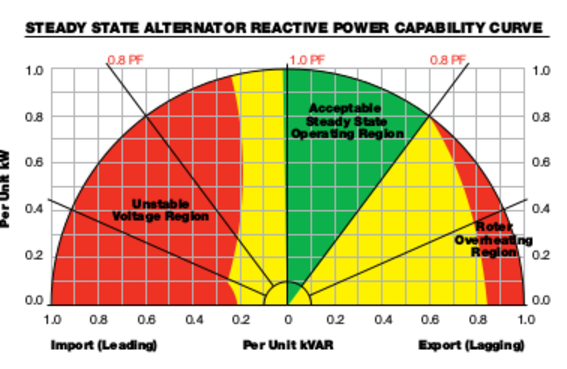
\includegraphics[width=6cm]{pf.pdf}
\pause

\dill{At low loads my powerfactor is bad, panic}
\end{frame}

\section{Diesels}
\begin{frame}\frametitle{Fuel Efficiency}
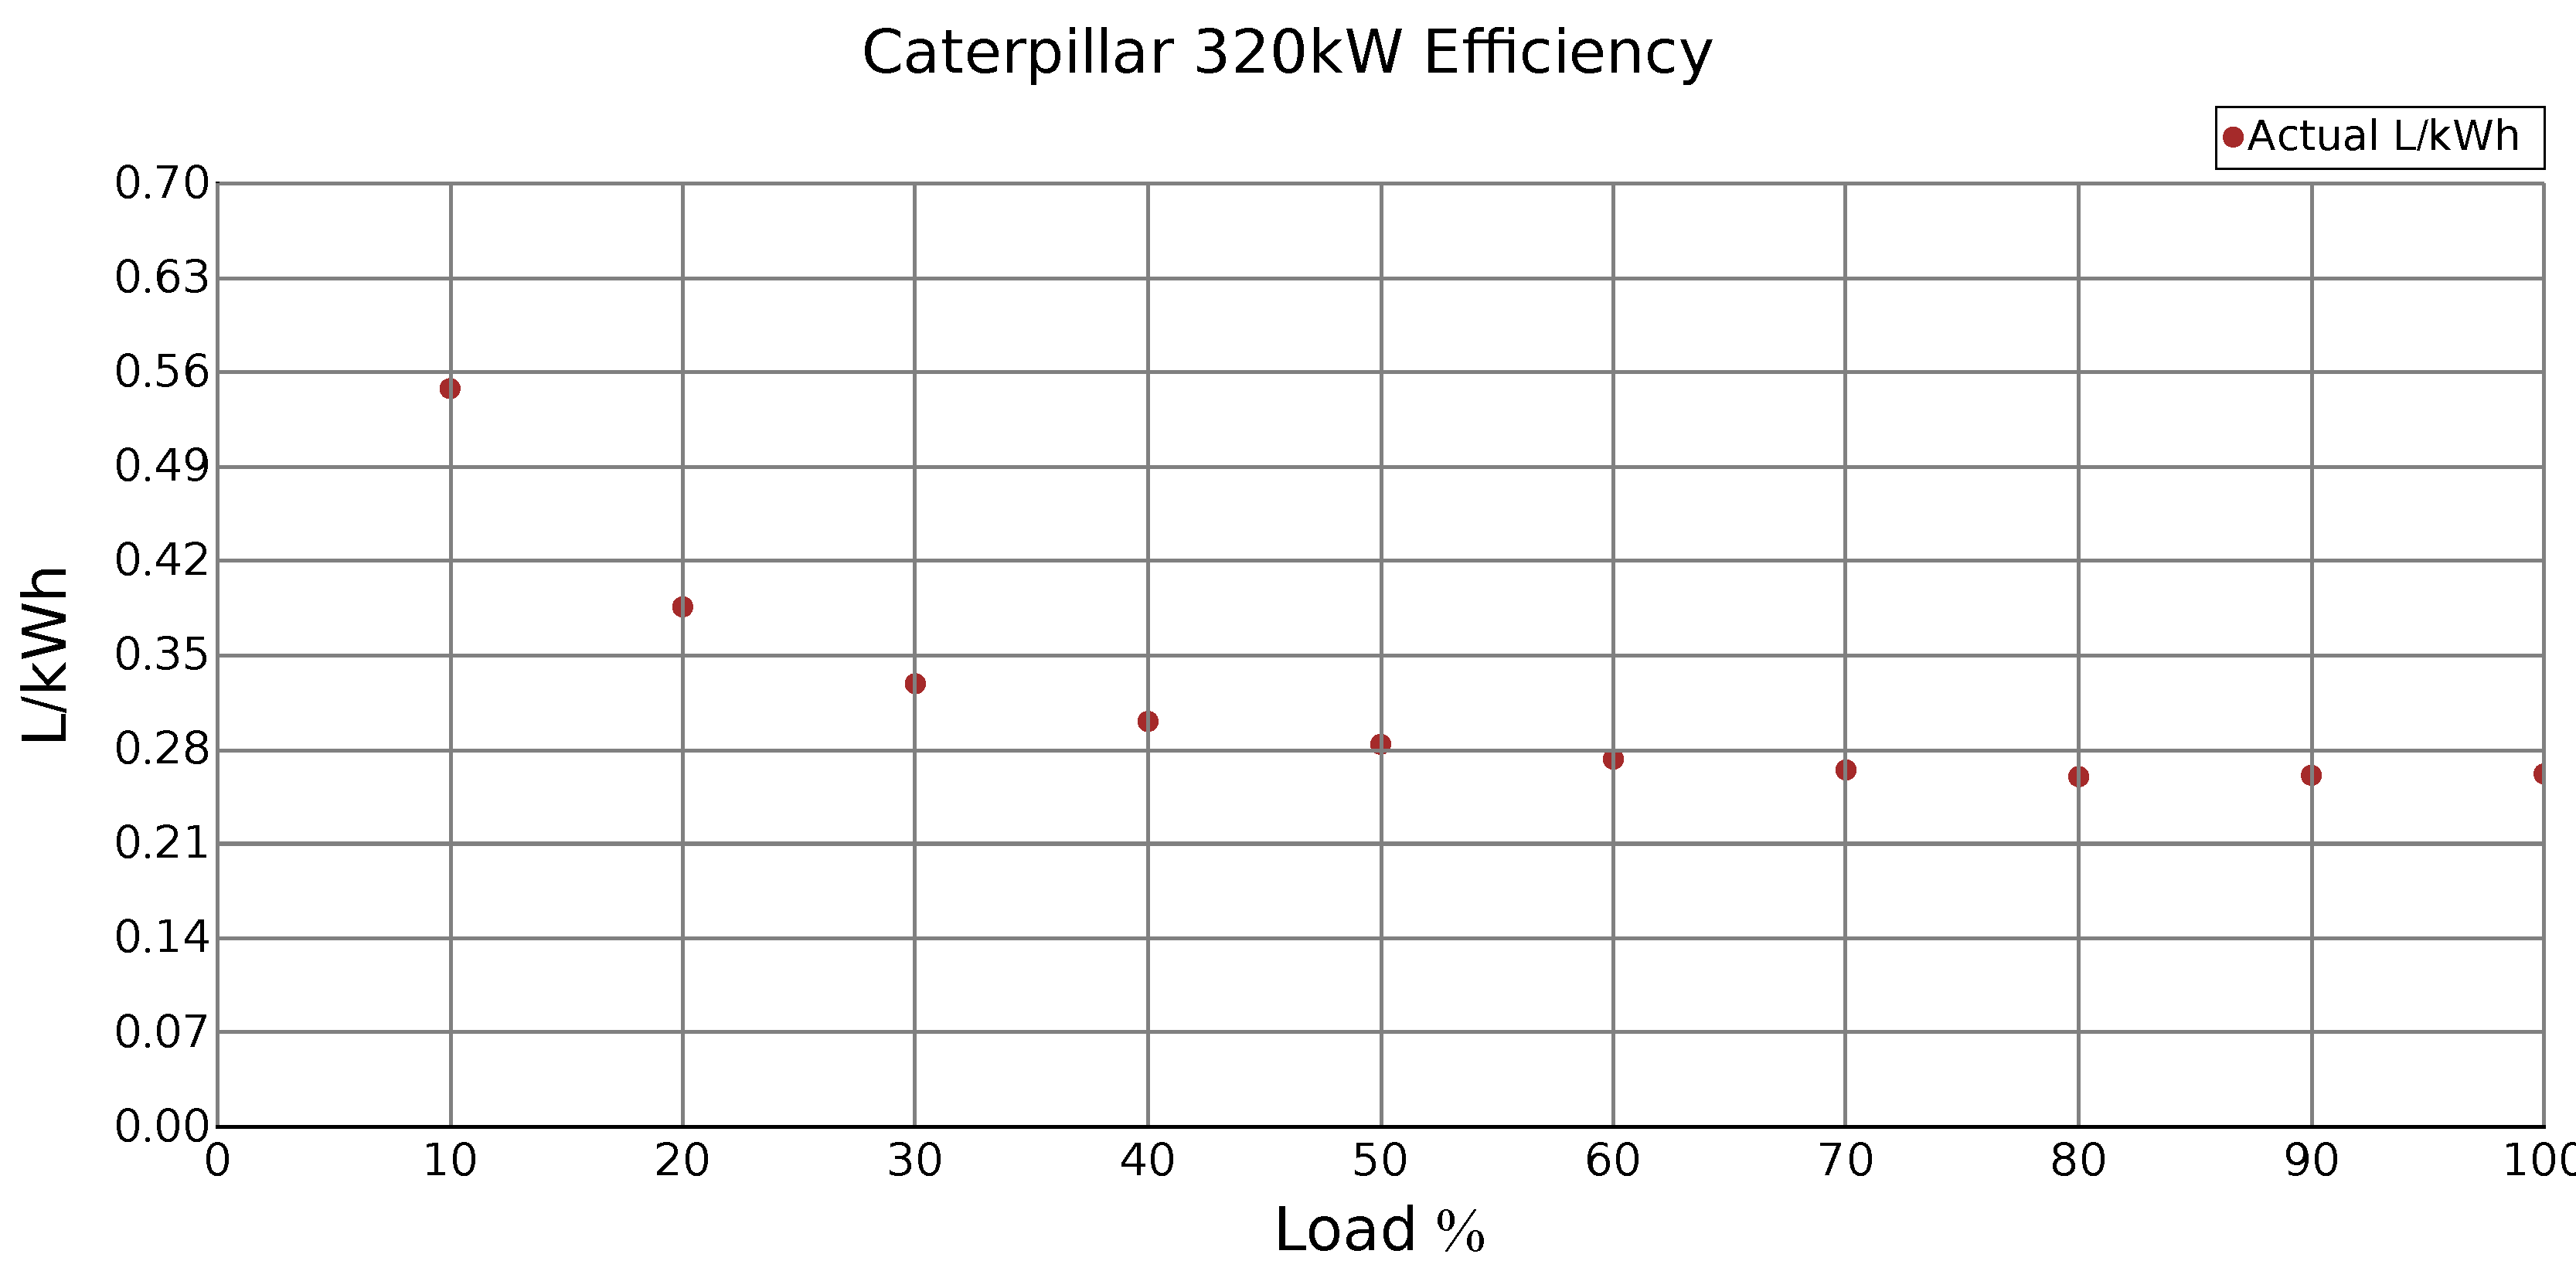
\includegraphics[width=10cm]{limits/figFuelCurve1.pdf}
\pause

\dill{So clearly we need to run diesels at around 80\% load 
  so they are efficient}
\end{frame}

\begin{frame}\frametitle{Fuel Consumption}
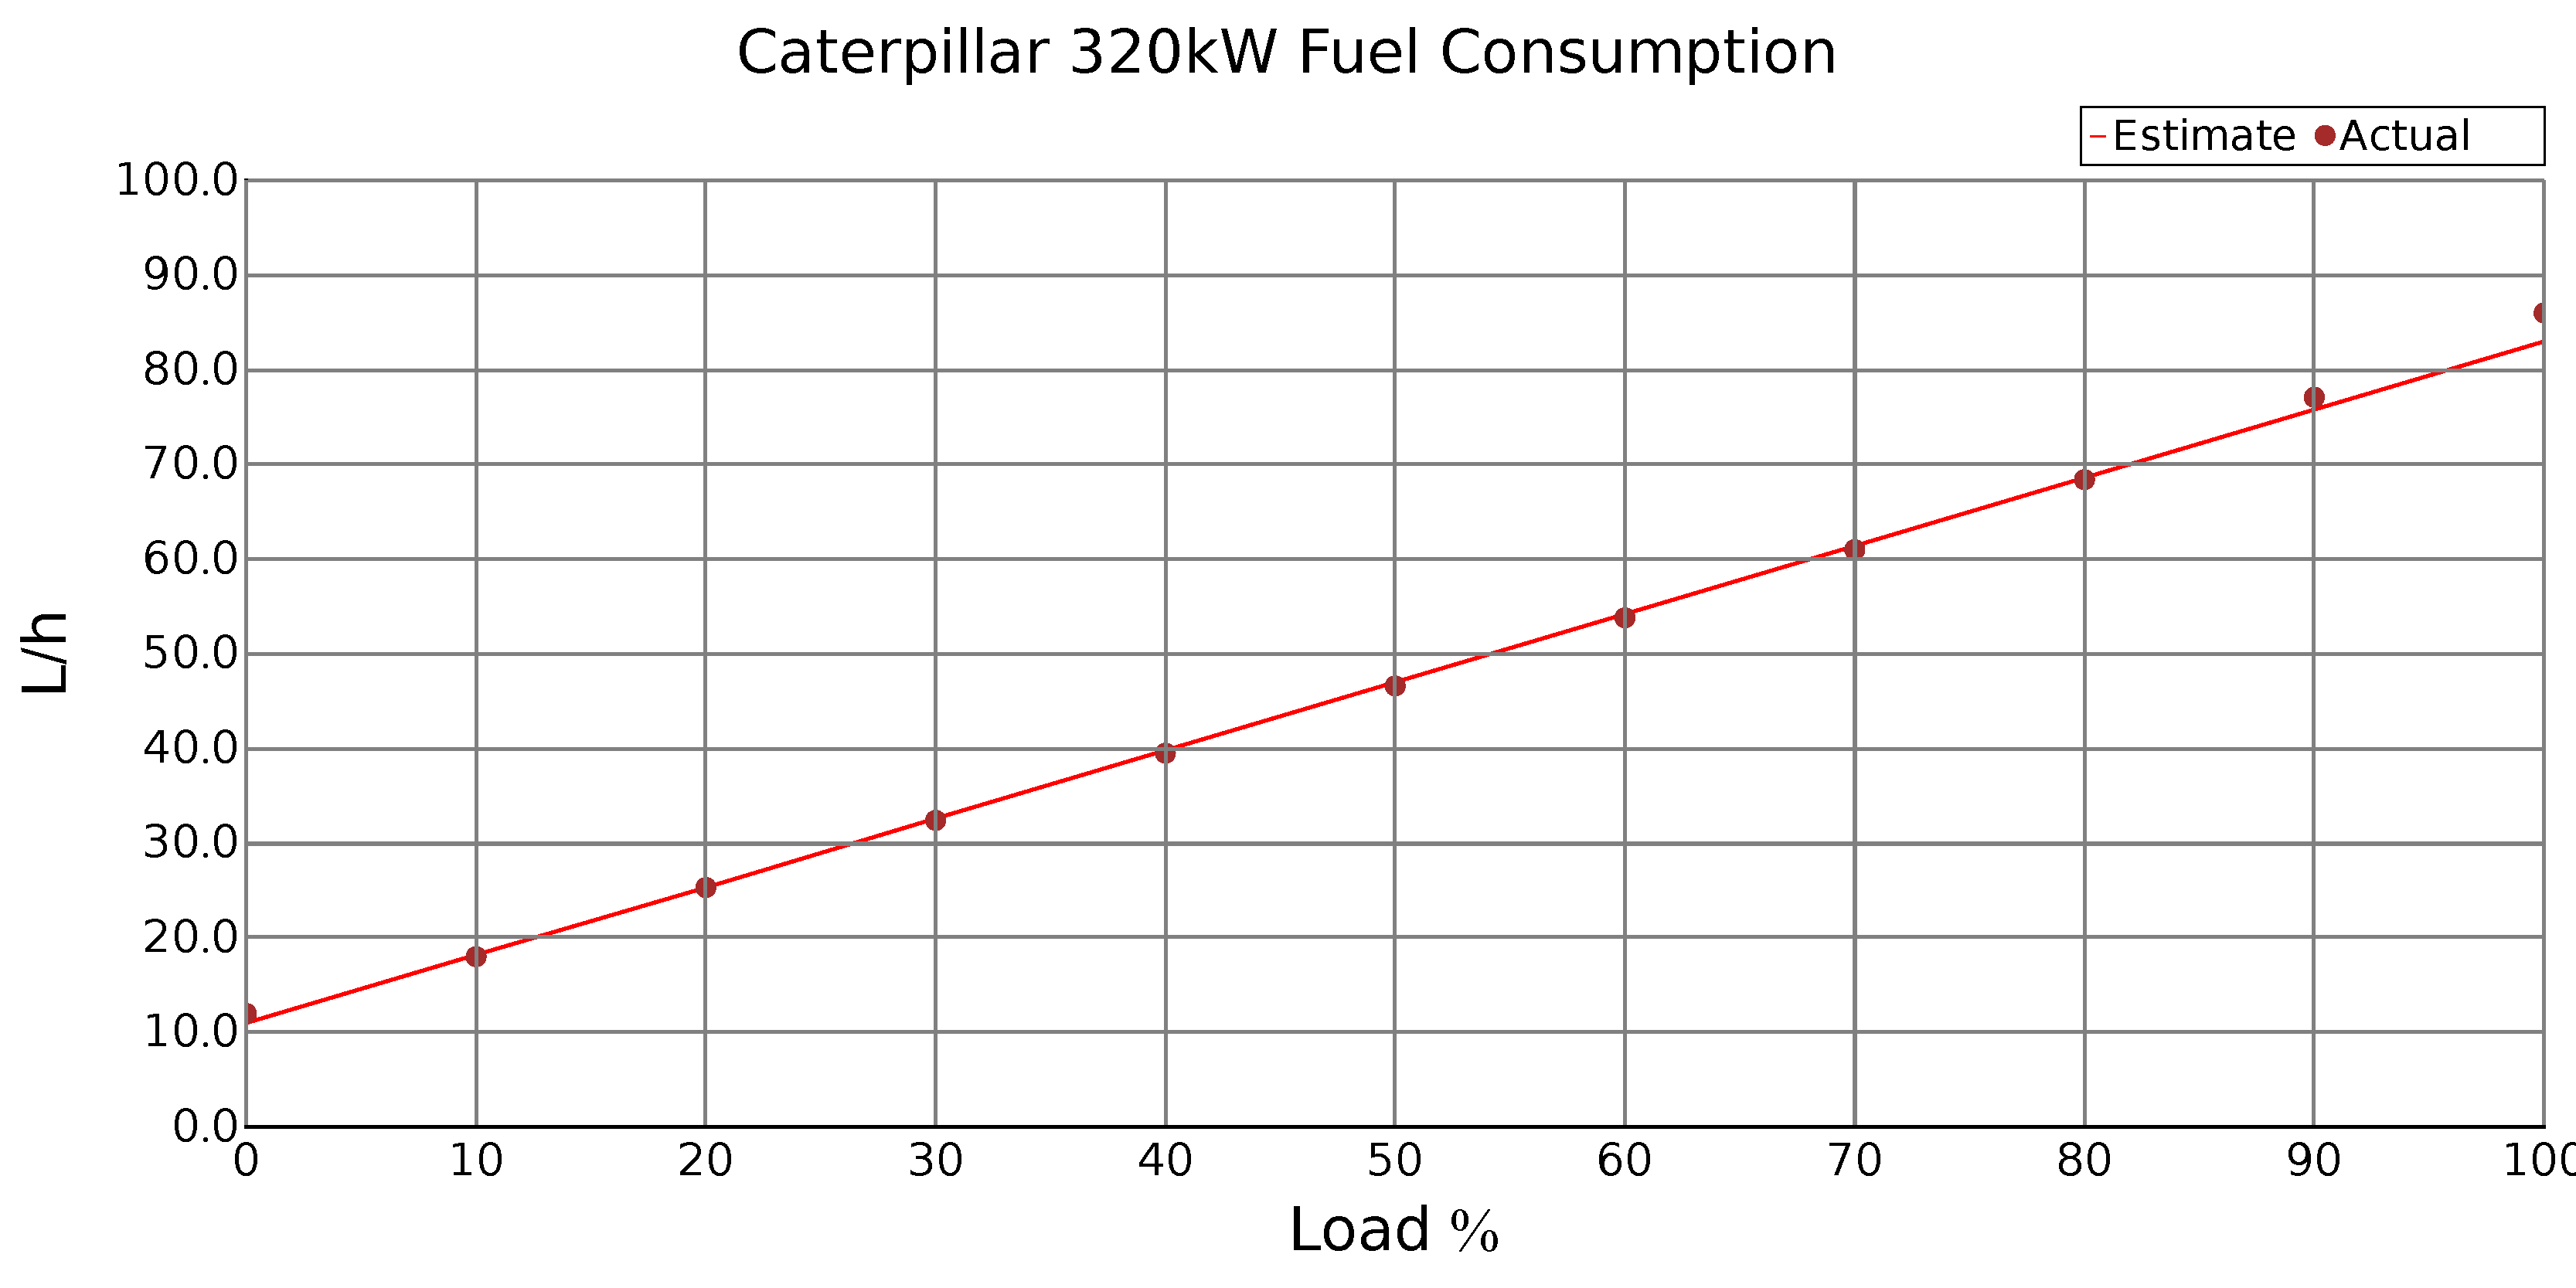
\includegraphics[width=10cm]{limits/figFuelCurve2.pdf}
\pause

\begin{itemize}
\item This makes sense since diesels run at fixed speed.
\pause
\item So there is a cost for spinning and a cost for generating.
\pause
\item So every bit of PV saves fuel, running a smaller generator
  saves fuel.
\end{itemize}
\end{frame}

\section{Others}
\begin{frame}\frametitle{Sky Camera Forecasting}
Use a SkyCamera to predict cloud over the next 2 minutes:
\pause
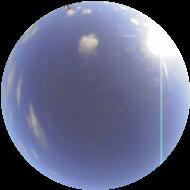
\includegraphics[width=4cm]{batch-2014-07-28T165557+0930-basis.jpg}
\pause

So you can run a smaller diesel: 2x320kW vs 1x320kW is around 30k\$/y.
\pause

Then start the next diesel when the cloud comes.
\end{frame}

\begin{frame}\frametitle{Demand Management}
Control \texttt{LoadP} so we can turn off some load, perhaps using:

\begin{description}
\item[Green Power Point] power iff there is excess green power.
\item[Brown Power Point] we assure power but there might be an outage
  for 2 minutes whilst we start a diesel.
\item[Red Power Point] always on.
\end{description}

The key thing is we need two way control and measurement.

See \href{http://www.saturnsouth.com}{Saturn South}
\end{frame}

\section{Conclusion}
\begin{frame}\frametitle{So what}
Note we've covered about 20 years research and development in
the last wee while.\pause

Feel free to finger poken the gentle speaker but also try to avoid the
dill tests.  \vfill \pause Finally:
\begin{quote}
“Learning is not compulsory...

\pause
neither is survival” -– W. Edwards Deming
\end{quote}
\end{frame}
\end{document}

